% Shared preamble for the supporting-information documents (S1-S5).
\documentclass[10pt,letterpaper]{article}
\usepackage[margin=1in]{geometry}
\usepackage{amsmath,amssymb}
\usepackage{booktabs,array,longtable}
\usepackage[table]{xcolor}
\usepackage{hyperref}
\usepackage{microtype}
\usepackage{listings}
\usepackage{graphicx}
\usepackage[labelfont=bf,labelsep=period,justification=raggedright,singlelinecheck=off]{caption}
\definecolor{linkblue}{HTML}{1C5CAB}
\definecolor{codebg}{HTML}{F4F4F1}
\hypersetup{colorlinks=true, linkcolor=linkblue, citecolor=linkblue, urlcolor=linkblue}
\lstset{basicstyle=\ttfamily\footnotesize, backgroundcolor=\color{codebg},
  frame=none, breaklines=true, columns=fullflexible, keepspaces=true,
  xleftmargin=4pt, xrightmargin=4pt, aboveskip=6pt, belowskip=6pt}
\setlength{\parindent}{0pt}
\setlength{\parskip}{5pt}
\raggedright
\renewcommand{\tablename}{Table}
\newcommand{\sititle}[2]{{\Large\bfseries #1}\par\vspace{3pt}{\large #2}\par\vspace{2pt}
  {\small\color{black!60}Supporting information for ``Environmental fluctuation limits gene regulation unless it can be tracked''}\par\vspace{10pt}}

\begin{document}
\sititle{S6 Text.}{EvoSim: connection count and wiring strength under fluctuation (exploratory)}

This study began with EvoSim, an individual-based model in which the genome is a
regulatory network of evolvable size (S1~Text). Its earlier results are
summarised in S4~Text. This experiment measured the strength of
regulatory connections as well as their number. It is exploratory. The
pre-registered confirmation could not be run (section 4), and EvoSim organisms
did not use the cue in this regime, so the experiment concerns fluctuation that
cannot be tracked. The main text reports the R-Aevol experiments.

\section*{1. Model}
\textbf{EvoSim} is an individual-based model of unicellular organisms on a
two-dimensional lattice with diffusing, cross-fed resources (S1~Text). Each genome is a gene regulatory network,
specified by a weight matrix and node biases, with 13 to 32 nodes. Thirteen
nodes are fixed. Twelve are read out as phenotypic traits (resource-uptake
allocation, body size, motility, division threshold, DNA repair, stress
tolerance and leakage) and one receives an abiotic cue, much like the sensor gene
of Sakamoto and Innan [1]. The remaining hidden
nodes are added by duplication and removed by deletion, so genome size can
evolve. The network is developed once at birth, and the phenotype does not
change afterwards. Mutation can create and remove connections and each non-zero
connection has a small maintenance cost, so connectivity is also free to evolve.

The design follows the R-Aevol experiments with an abiotic cue. Fluctuating
arms have an informative cue, a yoked cue decoupled from the environmental state
by running on an incommensurate period, or no cue. In a frozen environment the
cue is zero, so the three frozen arms are identical.

EvoSim is described in full, following the ODD protocol [2], in S1~Text; the
parts relevant to this experiment are summarised below. Organisms live on a
$G\times G$ lattice ($G=128$) with six diffusing resource channels. External
inflow, which varies seasonally, enters the first channel (with the exception
described under Environment and cue), and consuming channel $r$ releases a
byproduct into channel $r+1$, with yields declining along this chain. All arms
also experience rare random mass-mortality and famine events, on average one
every 25{,}000 time steps. Each organism
has an energy store and divides when the store exceeds a heritable threshold.
Starvation and the other causes of death are described in S1~Text.

\paragraph*{Genome and development.} A genome is a weight matrix $W$ and a bias
vector $b$ over $n_g$ nodes, with $13 \le n_g \le 32$. Nodes 1 to 12 are read out
as the phenotype, node 13 receives the abiotic cue, and hidden nodes
$14,\dots,n_g$ have no fixed meaning. Development takes place once, at birth.
Expression is initialised at 0.1 and updated eight times as
\begin{equation}
e_k \leftarrow \tanh\Big(b_k + \sum_m W_{mk}\, e_m + u_k\Big),
\end{equation}
where $u_k$ is the local concentration of resource $k$ for $k\le 6$, the cue for
$k=13$, and zero otherwise. The final expression values are mapped to the twelve
traits.

\paragraph*{Mutation.} At each birth, a Poisson number of point mutations with
mean $10^{-3} n_g^2$ is applied, each adding $\mathcal{N}(0,0.25^2)$ to a randomly
chosen weight. This rate is reduced by up to 85\% by the organism's heritable
repair trait. With probability equal to the reduced per-weight rate times $n_g$,
one node bias receives a mutation of the same size. The structural mutations are
gene silencing (probability 0.002), which sets a node's outgoing weights to zero;
gene duplication (0.002), which copies the regulatory role of one node onto
another and adds $\mathcal{N}(0,0.05^2)$ noise to every copied weight; and the
addition or deletion of a hidden node (0.003 each), where an added node is a
duplicate of an existing one made in the same way. Connection silencing
(probability 0.2 per birth) sets one randomly chosen weight to exactly zero.
Without it, additive mutation would drive density towards one. Each hidden node
costs 0.0015 and each non-zero weight $5\times10^{-5}$ energy units per time
step.

\paragraph*{Environment and cue.} An abiotic condition cycles through discrete
states with a period of 2{,}000 time steps. Each state changes which resource
channel gives the highest yield, and in fluctuating arms 40\% of the external
inflow goes to the favoured channel. In frozen arms all inflow enters channel 1,
which then also gives the highest yield. The phase of the cycle, scaled to $[-1,1]$, is the input to node 13 and
identifies the current state. Fluctuating arms have six states and frozen arms
one. In the yoked arm the cue is instead the phase multiplied by
$10/\varphi\approx6.18$, with $\varphi$ the golden ratio, and wrapped back into
the same range, so that it takes the same values but carries only 0.0004 bits of
information about the state. In the no-cue arm the gain of the cue is
zero. With a single state the cue is identically zero, so the three frozen arms
produce identical runs and were analysed as one arm.

\paragraph*{Measures.} For every organism at birth we record the number of
weights with $|w|>10^{-4}$, the strength density $\sum|w|/n_g^2$ over all $n_g^2$
weights, including zeros, and $n_g$. The log holds their population means at
each time step. Count density is the mean number of non-zero weights divided by
the squared mean $n_g$, and total strength is the mean strength density
multiplied by the squared mean $n_g$. Each measure is then averaged over the
last 20\% of the run. Populations
that went extinct were excluded and their number is reported.

\paragraph*{Runs.} We ran six arms with 30 seeds each for 150{,}000 time steps
(180 runs), about 6{,}200 generations in fluctuating and 4{,}900 in frozen
populations (24 and 31 time steps per generation, from the slope of mean lineage
depth). Runs are deterministic for a given seed and, on the same machine
and Julia version, bit-identical across thread counts (checked at 1, 4 and 8
threads).

\section*{2. Results}
Earlier EvoSim experiments had found that fluctuation increases connection
density (S4~Text). We repeated the comparison in 180 runs (six arms of 30 seeds,
150{,}000 time steps each) and measured the strength of connections as
well as their number. The cue is zero in a frozen environment, so the three frozen arms are
identical and the runs contain 120 distinct populations. Without a cue,
fluctuation raised count density, the
proportion of possible connections that are non-zero, from 0.467 to 0.587
($+25.5\%$, $p<10^{-4}$, $d=2.2$; 28 surviving fluctuating and 30 frozen
populations; Fig AA), and the number of non-zero connections from 86
to 120 ($+39\%$, $p<10^{-4}$). Total wiring strength did not change (38.0 in
frozen and 37.5 in fluctuating populations, $p=0.86$; Fig AC).
Fluctuating networks thus had more connections but not more wiring, and the
average non-zero connection was about 30\% weaker. Strength density, the summed
absolute weight divided by the number of possible connections, fell from 0.207
to 0.184 ($-10.9\%$, $p<10^{-4}$, $d=-1.4$; Fig AB), mostly because
there were more possible connections. Node count stayed close to its minimum of
13 in this regime and increased only slightly ($+0.6$ nodes, $p=0.047$), which
raises $n_g^2$ by about 9\%. With the informative and the yoked cue, fluctuation
had effects in the same directions (count density $+18\%$ and $+28\%$, total
strength unchanged, $p=0.40$ and $0.59$).

Population size is a possible confound. Fluctuating populations were 40\% smaller than frozen ones, as expected since in frozen dishes
all inflow feeds the best-paying channel (S1~Text), and population size can change
genome architecture by itself. Because the population sizes of the two arms did not
overlap, the two effects cannot be separated statistically, and the
correlations within arms point in different directions for the two measures.
Larger populations had lower strength density in every arm ($r$ between $-0.31$
and $-0.47$; Fig AD), so population size would predict higher strength
density in the smaller fluctuating populations, the reverse of what we found.
Count density, in contrast, was higher in smaller populations within each
fluctuating arm ($r$ between $-0.63$ and $-0.72$), though not in the frozen arm
($r=0.24$), so population size may contribute to the increase in connection
number. The cue was also not used in this regime. Populations with the informative and
the yoked cue were the same size ($p=0.79$) and had the same strength density
($p=0.99$), although count density was lower with the informative cue (0.55
against 0.60, $p=0.009$). EvoSim organisms respond to the cue only when
development is reversible, and even then they match their phenotype to the
current state only in part (S4~Text). The EvoSim results
concern fluctuation that the organisms cannot track.

\begin{figure}[!ht]
\centering
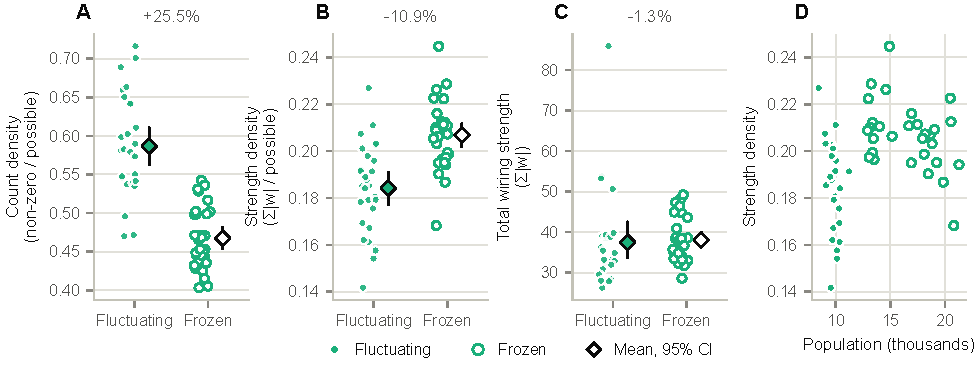
\includegraphics[width=\linewidth]{../figures/fig2_evosim.pdf}
\caption*{{\bf Fig A. EvoSim: more connections, no more wiring.}
Fluctuating (no cue; filled) versus frozen (hollow) populations, one point per
population; diamonds are means with bootstrap 95\% confidence intervals. Numbers
above panels are the change in the mean.
(A) Count density, the number of non-zero connections divided by the number of possible connections.
(B) Strength density, the summed absolute weight divided by the number of possible connections.
(C) Total wiring strength.
(D) Strength density against population size within each arm. Extinct
populations (2 of 30 fluctuating, 0 of 30 frozen) are excluded.}

\end{figure}

\section*{3. Interpretation}
Gene duplication and node addition copy the connections of an existing node and
add small random values to every copied weight, including weights that were zero,
so each duplication can create many weak connections. Point mutations that hit a
zero weight also create connections. If purifying selection is weaker in the
smaller populations of fluctuating environments, such connections would persist
and connection number would rise without an increase in total strength, which
fits the correlations with population size within the fluctuating arms. We have
not tested this mechanism.

\section*{4. Limitations and the confirmation that was not run}
Fluctuation and population size are confounded between arms. The within-arm
correlations argue against population size as the cause of the lower strength
density but are consistent with a contribution to the higher connection count.
We pre-registered a confirmation of the divergence between count and strength
(P5; commit \texttt{4bc16c3}) in a regime with more hidden nodes, on condition
that fluctuating and frozen populations survived a viability pilot there.
They did not (2 to 5 of 6 fluctuating populations survived at grids 80, 96 and
112, compared with 6 of 6 frozen populations; commit \texttt{56fe3a0}), so the
confirmation was not run and the result remains exploratory.

\section*{References}
\small
\begin{enumerate}\setlength{\itemsep}{1pt}
\item Sakamoto T, Innan H. On the evolutionary origin of discrete phenotypic plasticity. G3 (Bethesda). 2024;14(9):jkae144.
\item Grimm V, Railsback SF, Vincenot CE, Berger U, Gallagher C, DeAngelis DL, et al. The ODD protocol for describing agent-based and other simulation models: a second update to improve clarity, replication, and structural realism. J Artif Soc Soc Simul. 2020;23(2):7.
\end{enumerate}

\end{document}
